\documentclass[9 pt]{beamer}
\usepackage{graphics}
\usepackage{xcolor}
\usepackage{array}
\usepackage[utf8]{inputenc}
\renewcommand\fbox{\fcolorbox{purple}{white}}
\usepackage{amsmath,accents}
\usepackage{tikz}

\usetikzlibrary{angles, quotes, calc, decorations.markings, intersections}
\newcommand{\midlabelline}[3]{
	\node (midlabel) at ($ (#1)!.5!(#2) $) {#3};
	\draw[<-] (#1) --  (midlabel);
	\draw[->] (midlabel) -- (#2);
}
\newcommand{\pa}{\partial}
\newcommand{\mcm}[1]{\mathcal{#1}}
\newcommand{\bo}{\mcm{O}}
\newcommand{\sDelta}{{\scriptstyle \Delta}}
\newcommand{\gs}{\hspace{0.35cm}}
\newcommand{\mvec}[1]{\accentset{\rightharpoonup}{#1}}

\usepackage{import}
\usetheme{Frankfurt}
\title{Finite Difference Method For Poisson Equation}
\date{\today}
\author{Akarsh Shukla , Brahmanand Mishra and Shashvat Jain}

\begin{document}
\maketitle

\section{Content}
	\begin{frame}{Talk}
			\begin{block}{Plam}
				\begin{itemize}
					
					\item We will start the talk by \alert{introducing} our topic.
					\item After introdudcing the topic, we would like to exaplain our \alert{ question}. 
					\item Then we will proceed to describe the various \alert{methods} we have used in the project.
					\item After discussion on methods, we would like to discuss our \alert{results}.
					\item We will conclude the talk with \alert{conclusion} of results and by sharing our \alert{experience} in completing this project.
					
				\end{itemize}
			\end{block}
		
	\end{frame}

\section{Introduction}
	\begin{frame}{Introduction}
		\begin{itemize}
			\item  Poisson Equation is an \alert{elliptic} partial differential Equation.having general form as -: 
			\begin{center}
				\setlength\fboxrule{2pt}\setlength\fboxsep{2mm}
				\fbox{$ \frac{\partial^2 u}{\partial x^2} + \frac{\partial^2 u}{\partial y^2} =  f({r}) $}
			\end{center}
			\item Differetial Equation can be solved by variety of methods such as spectral methods, finite element methods, FDI. 
			\item Method of finite differences converts differential Equation   into a system of linear equation by approxiamting the derivatives using taylor series. 
			\item This system of linear equation obtained can be solved in two ways to obtain the solution of  differential equation-:
				\begin{itemize}
					\item Implicit Methods
					\item Explicit Methods
				\end{itemize}
			
			\item Implicit methods include many iterative schemes which can be employed to solve this system of linear equation such as \alert{Gauss Seidel, SOR} and \alert{Jacobi Method}.
		
		\end{itemize}
		
	\end{frame}

\section{Theory}
	\subsection{Problem}
	\begin{frame}{Theory}
		\section{Problem}
		The below figure shows an interleaved capacitor -:
			\begin{figure}[h]
			\centering
			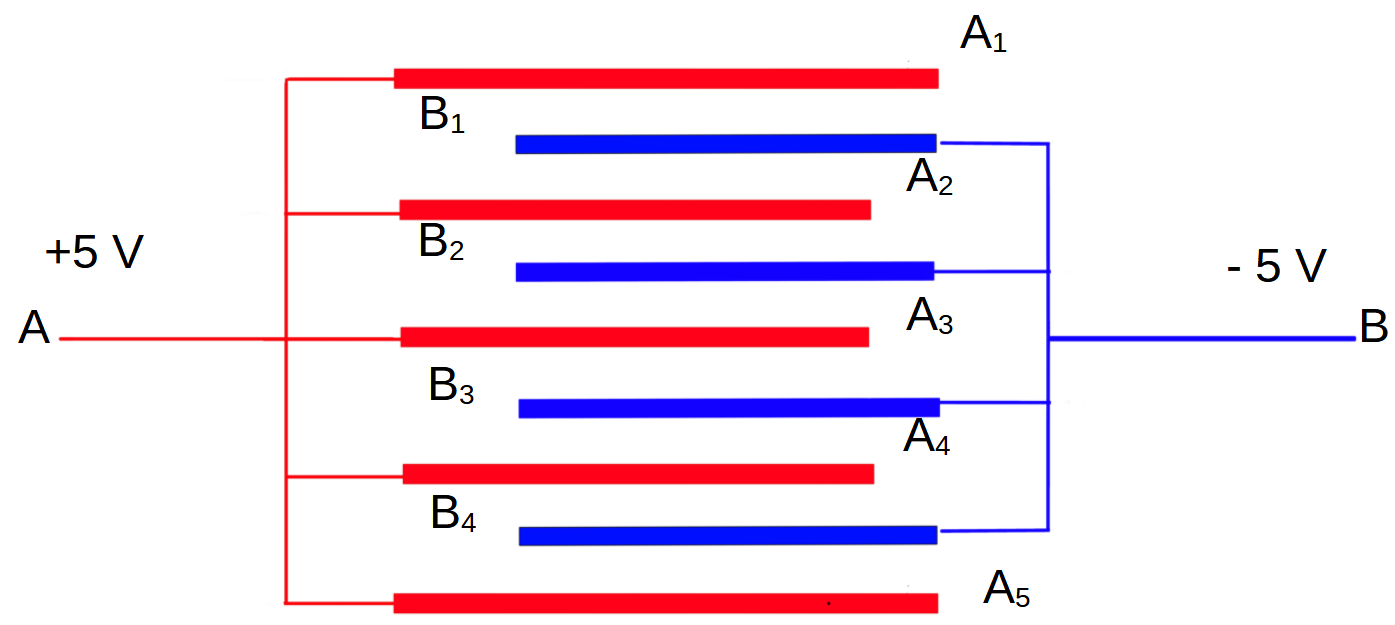
\includegraphics[width=2cm, height=1.9cm]{insert.png}
			\caption{\small Diagram dipciting the arrangement of plates in a interleaved fashion.}
			\label{fig 1: the capacitor}

			\end{figure}
			After non -dimensionalising we had following poisson equation-:
			$$ \frac{\partial^2U'(x',y') }{\partial x^{'2}} + \frac{\partial^2U'(x',y') }{\partial y^{'2}}= -\frac{\rho'(x',y') s^2}{\epsilon_0 \nu} $$
			
		\end{frame}
	\begin{frame}{Problem}
		\begin{equation}
			\rho'(x',y') =  \begin{cases}
				-2\epsilon_0 \times 10^5  & :\text{if} \; (x',y') \in B_i \; \text{where} \; i = 1,2,3,4 \\
				2\epsilon_0 \times 10^5 & :\text{if} \; (x',y') \in A_i \; \text{where} \; i = 2,3,4 \\
				0  & : \; \text{elsewhere}
			\end{cases}
		\end{equation}
		With boundary conditions as -:
		\begin{align}
			& U(0,y) = +5/\nu \quad \ U(4,y) = +5/\nu \\ 
			& U_y(x,0) = 0 \qquad \ U_y(x,4.4) = 0 
		\end{align}
		
		\end{frame}	
	\section{Methodology}
	\begin{frame}{Methodology}
		\subsection{Finite Differences}
		\begin{itemize}
			\item Finite Difference converts PDE into difference equation.
			\item Domain is converted into a mesh of equidistant grid points.
			\item Taylor series is used to approximate the value at  these grid points.
			 \item After using Finite Difference operators we get the following stencil for poisson equation
		\end{itemize}
		\begin{align}
			U_{i,j} = \frac{1}{4} \left[ U_{i+1,j}+ U_{i-1,j} + U_{i,j+1}+ U_{i,j+1} + h^2\frac{\rho'_{i,j} s^2}{\epsilon_0 \nu} \right]
		\end{align}
		This stencil can be represented with the help of following diagram -: \\
		\begin{figure}
			\centering
			
			\scalebox{0.4}{[
				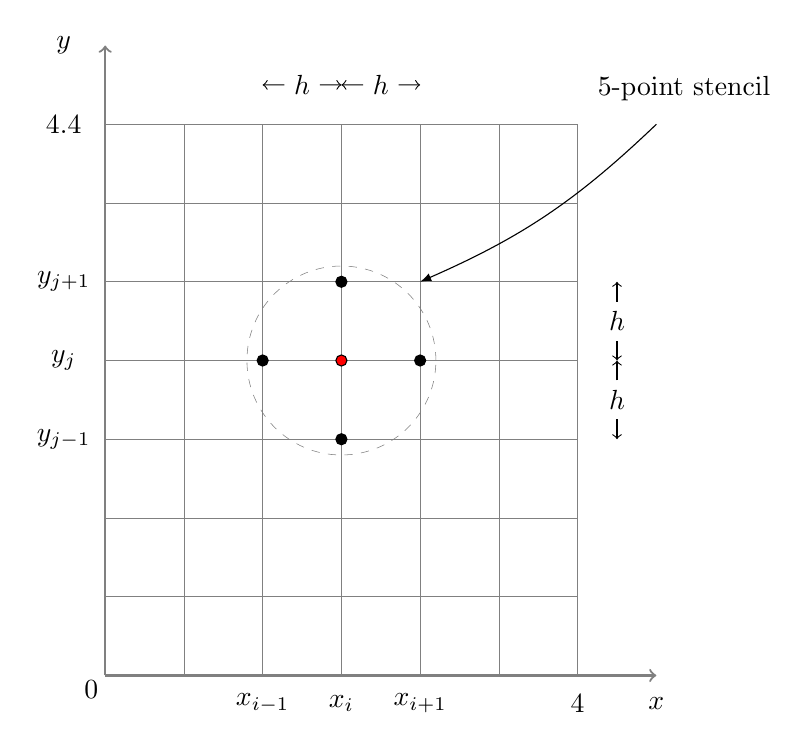
\begin{tikzpicture}
				\coordinate (Y) at (-15pt,8);
				\coordinate (X) at (7,-10pt);
				\draw[step = 1cm,gray, very thin] (0,0) grid (6,7);
				\draw[thick,color=gray,->] (0,0) -- (7,0);
				\draw[thick,color=gray,->] (0,0) -- (0,8);
				\draw (X) node {$x$};
				\draw (Y) node {$y$};
				\draw (X) node[shift={(-4,0)}] {$x_i$};
				\draw (Y) node[shift={(0,-4)}] {$y_j$};
				\draw (X) node[shift={(-5,0)}] {$x_{i-1}$};
				\draw (Y) node[shift={(0,-5)}] {$y_{j-1}$};
				\draw (X) node[shift={(-3,0)}] {$x_{i+1}$};
				\draw (Y) node[shift={(0,-3)}] {$y_{j+1}$};
				\draw (Y) node[shift={(0,-1)}] {$4.4$};
				\draw (X) node[shift={(-1,0)}] {$4$};
				\midlabelline{[shift={(-0.5,3cm + 10pt)}]X}{[shift={(-0.5,4cm +10pt)}]X}{$h$};
				\midlabelline{[shift={(-0.5,4cm +10pt)}]X}{[shift={(-0.5,5cm +10pt)}]X}{$h$};
				\coordinate (Xa) at ([shift={(2cm +15pt,-0.5)}]Y); 
				\coordinate (Xb) at ([shift={(3cm +15pt,-0.5)}]Y); 
				\coordinate (Xc) at ([shift={(4cm +15pt,-0.5)}]Y); 
				\midlabelline{Xa}{Xb}{$h$};
				\midlabelline{Xb}{Xc}{$h$};
				\draw (0,0) node[shift={(-5pt,-5pt)}] {$0$};
				\draw[fill=red] (3,4) circle (2pt) ;
				\draw[fill=black] (4,4) circle (2pt) ;
				\draw[fill=black] (2,4) circle (2pt) ;
				\draw[fill=black] (3,3) circle (2pt) ;
				\draw[fill=black] (3,5) circle (2pt) ;
				\draw[dashed,very thin,color=gray] (3,4) circle (1.2cm) ;
				\draw [latex-] (4cm,5cm) to [bend right=10] (7,7) node[anchor=south,shift={(10pt,5pt)}] {$5$-point stencil};
			\end{tikzpicture}]}
		\end{figure}
		\end{frame}	
		\subsection{Truncation Error}
		\begin{frame}{Truncation Error}
			\begin{itemize}
				\item Truncation Error arises due to truncation of Taylor series used for approximating the value of derivative to form a difference equation.
				\item First order derivative can be approximated in three ways-:
					\begin{itemize}
						\item Forward Difference Method
						\item Backward Difference Method
						\item Central Difference Method \\
						\medskip
					\end{itemize}
				
						\begin{center}
							
							\begin{tabular}{ || c| c || } 
								\hline 
								Forward Difference Method &  $ \mcm{O}(\Delta x)$ \\ 
								\hline 
								Backward Difference Method &$ \mcm{O}(\Delta x)$  \\ 
								\hline 
								Central Difference Method &  $ \mcm{O}((\Delta x)^2) $ \\ 
								\hline \hline
							\end{tabular}
						\end{center}
						\item Above table shows that central order approximation are more accurate than one sided differences.
						\item Second Order derivative is also second order accurate.
				
			\end{itemize}
		\end{frame}
		\subsection{Iterative Method }
		\begin{frame}{Iterative Method}
			\begin{itemize}
				\item Iterative methods are techniques that exploit the properites of system to solve it implicitly to make computation faster.
				\item We have used following iteratiion schemes-:\\
			
					 \begin{block}{Jacobi Method}
						This method starts with a guess value and with each iteration, it replace guess values with new obtained values from iteration.$$ x^{(n+1)}_{i,j} = S(X^{(n)},P,h,i,j) $$
						\end{block}
					 \begin{block}{Gauss Seidel Method}
						This method uses the obtained value in the same iteration for other unknowns.$$x^{(n+1)}_{i,j} = S(X^{(n+1)},P,h,i,j)$$
						\end{block}
					
					\begin{block}{SOR}
							This method involves a relaxation factor (greater than 1) which is multiplied to values obtained from Gauss Seidel before replacing old values.$$x^{(n+1)}_{i,j} = x^{(n)}_{i,j}+ \omega(S(X^{(n+1)},P,h,i,j)- x^{(n+1)}_{i,j})$$
							
						\end{block}
				
					
					\end{itemize}
				\end{frame}
			\section{result}
				\subsection{Expectation}
				\begin{frame}{Expectation}
					We expect the following graph-:\\
					\begin{itemize}
						\item $ \alpha_1 $ should decrease from positive to negative potential
						\item $ \alpha_2 $ should have negatively charged potential
						\item $ \alpha_3 $ should increase from negative to positive potential
						\item $ \alpha_4 $ should have positively charged  potential
					\end{itemize}
					
				\end{frame}
				\subsection{Numerical Result}
				\begin{frame}{Numerical Result}
					We obtained following graphs as solution -: \\
					
				\end{frame}
				\section{Conclusion}
					\begin{frame}{Conclusion}
						\begin{block}{Result}
							\begin{itemize}
								\item After computing thte problem of interleaved capacitor from three different iterative schemes, we have arrived at the conclusion that SOR is the fastest among three.
							\end{itemize}
							\end{block}
						\begin{block}{Experiences}
							\begin{itemize}
								\item We have gained more intuition and it has helped us to grasp the concept of electrostatic potential.
								\item We have learnt a lot of new techniques and methods related to computational solution of differential equation.
								\item There are some techniques and methods which we could not implemnet  but surely they have given us some things to ponder upon in future.
								\item This project has also  introduced us to delight of finding out new things as most of things we did in this project were completely new to us.
							\end{itemize}
						\end{block}
							
					\end{frame}
				\begin{frame}{References}
					
					content...
				\end{frame}
\end{document}

